\documentclass[12pt, twoside]{article}
\usepackage[francais]{babel}
\usepackage[T1]{fontenc}
\usepackage[latin1]{inputenc}
\usepackage[left=7mm, right=7mm, top=7mm, bottom=7mm]{geometry}
\usepackage{float}
\usepackage{graphicx}
\usepackage{array}
\usepackage{multirow}
\usepackage{amsmath,amssymb,mathrsfs}
\usepackage{soul}
\usepackage{textcomp}
\usepackage{eurosym}
 \usepackage{variations}
\usepackage{tabvar}


\pagestyle{empty}

\begin{document}


\section*{\center{Correction devoir surveill� 6}}


\subsection*{Exercice 3}



  
  \begin{tabular}{c|c}
\begin{minipage}{10cm}
 1.  \ul{M�thode 1:} Aire(EFG)= Aire(EUF)+ Aire (EUG)

\enskip

\quad \quad \quad \qquad \qquad \qquad \quad \quad = $\dfrac{EU \times
FU}{2}+\dfrac{EU \times UG}{2}$

\medskip

\textbf{sujet 1:}  Aire (EFG)=$\dfrac{3,7 \times 4}{2}+\dfrac{3,7 \times 2}{2}=11,1cm^2$

\medskip

\textbf{sujet 2:}  Aire (EFG)=$\dfrac{3,5 \times 6}{2}+\dfrac{3,5 \times 3}{2}=15,75cm^2$
\end{minipage}
&
\begin{minipage}{8cm}
\ul{M�thode 2:} \quad FG=FU+UG

\enskip

Aire(EFG)=$\dfrac{EU \times FG}{2}$

\medskip

\textbf{sujet 1:} Aire(EFG)=$\dfrac{3,7 \times 6}{2}=11,1cm^2$

\medskip

\textbf{sujet 2:}  Aire(EFG)=$\dfrac{3,5 \times 9}{2}=15,75cm^2$
\end{minipage}
\end{tabular}  

\bigskip


2. Aire(ABC)=$\dfrac{AB \times AC}{2}=\dfrac{8 \times 6}{2}=24cm^2$.


\subsection*{Exercice 4}

\begin{tabular}{c|c}
\begin{minipage}{9cm}
\textbf{sujet 1}: Aire(DBC)=$\dfrac{DC \times BH}{2}$

\enskip

En rempla�ant: 10,5=$\dfrac{7 \times BH}{2}=3,5 \times BH$

\enskip

Donc $BH=\dfrac{10,5}{3,5}=3cm$.
\end{minipage}
&
\begin{minipage}{9cm}
\textbf{sujet 2}: Aire(DBC)=$\dfrac{DC \times BH}{2}$

\enskip

En rempla�ant: 49,5=$\dfrac{11 \times BH}{2}=5,5 \times BH$

\enskip

Donc $BH=\dfrac{49,5}{5,5}=9cm$.
\end{minipage}
\end{tabular}


\subsection*{Exercice 5}

\begin{tabular}{cc}
\begin{minipage}{6cm}
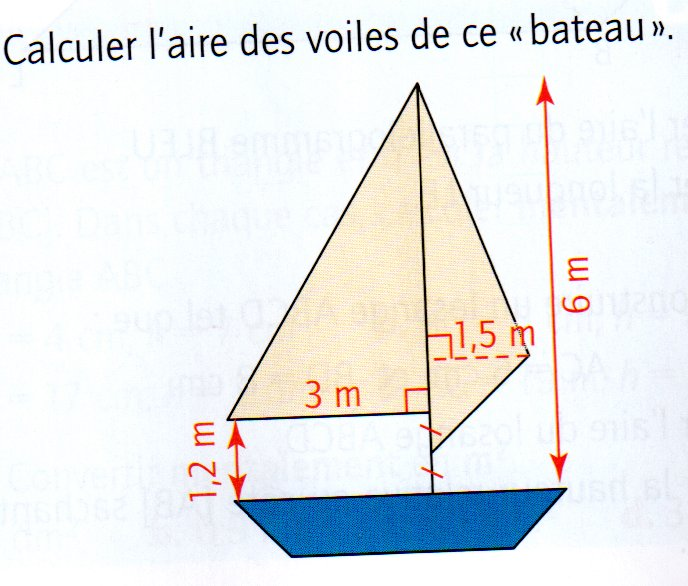
\includegraphics[width=6cm]{images/ex5.jpg}
\end{minipage}

&

\begin{minipage}{12cm}
On sait que: CF=1,2m, AF=6m, BC=3m, GD=1,5m.

\enskip

D'apr�s le codage, E est le milieu de [CF] donc CE=EF=0,6m.
 
\enskip

Calcul de AC: AC=AF-CF=6-1,2=4,8

\enskip

Calcul de AE: AE=AF-EF=6-0,6=5,4

\enskip

$\bullet$ Aire(ABC)=$\dfrac{BC \times CA}{2}=\dfrac{3 \times 4,8}{2}=7,2m^2$




\enskip


$\bullet$ Aire(ADE)=$\dfrac{GD \times AE}{2}=\dfrac{1,5 \times 5,4}{2}=4,05m^2$





\enskip

$\bullet$ Aire(voile)=Aire(ABC)+Aire(ADE)=7,2+4,05=11,25$m^2$
\end{minipage}
\end{tabular}

\subsection*{Exercice 6}

\begin{tabular}{l|l}
\begin{minipage}{9cm}

\textbf{sujet 1:}

\enskip

$C=\dfrac{2}{5}+\dfrac{3}{10}=\dfrac{4}{10}+\dfrac{3}{10}=\dfrac{7}{10}$

\medskip

$D=\dfrac{5}{6}-\dfrac{1}{12}=\dfrac{10}{12}-\dfrac{1}{12}=\dfrac{9}{12}$

\medskip

$E=4+\dfrac{3}{5}=\dfrac{4}{1}+\dfrac{3}{5}=\dfrac{20}{5}+\dfrac{3}{5}=\dfrac{23}{5}$

\medskip

$F=\dfrac{7}{3}+\dfrac{5}{9}-2=\dfrac{21}{9}+\dfrac{5}{9}-\dfrac{2}{1}=\dfrac{26}{9}-\dfrac{18}{9}=\dfrac{8}{9}$
\end{minipage}
&
\begin{minipage}{9cm}
\qquad \textbf{sujet 2:}

\enskip

\qquad $C=\dfrac{2}{6}+\dfrac{3}{12}=\dfrac{4}{12}+\dfrac{3}{12}=\dfrac{7}{12}$

\medskip

\qquad $D=\dfrac{7}{10}-\dfrac{1}{5}=\dfrac{7}{10}-\dfrac{2}{10}=\dfrac{5}{10}$

\medskip

\qquad $E=3+\dfrac{5}{7}=\dfrac{3}{1}+\dfrac{5}{7}=\dfrac{21}{7}+\dfrac{5}{7}=\dfrac{26}{7}$

\medskip

\qquad $F=\dfrac{7}{4}+\dfrac{5}{2}-3=\dfrac{7}{4}+\dfrac{10}{4}-\dfrac{3}{1}=\dfrac{17}{4}-\dfrac{12}{4}=\dfrac{5}{4}$
\end{minipage}
\end{tabular}

\end{document}
